% LaTeX rebuttal letter example. 
% 
% Copyright 2019 Friedemann Zenke, fzenke.net
%
% Based on examples by Dirk Eddelbuettel, Fran and others from 
% https://tex.stackexchange.com/questions/2317/latex-style-or-macro-for-detailed-response-to-referee-report
% 
% Licensed under cc by-sa 3.0 with attribution required.
% See https://creativecommons.org/licenses/by-sa/3.0/
% and https://stackoverflow.blog/2009/06/25/attribution-required/

\documentclass[11pt]{article}


\usepackage[utf8]{inputenc}
%\usepackage{lipsum} % to generate some filler text
\usepackage{fullpage}

\usepackage{color}
\usepackage{todonotes}

% import Eq and Section references from the main manuscript where needed
% \usepackage{xr}
% \externaldocument{manuscript}






%%%%%%%%%%%%%%ANSWERS TO REVIEWRS



\newcommand{\hl}[1]{\colorbox{yellow}{#1}}
\newcommand{\hldone}[1]{\colorbox{green}{#1}}
\newcommand{\hldoing}[1]{\colorbox{cyan}{#1}}


% package needed for optional arguments
\usepackage{xifthen}
% define counters for reviewers and their points
\newcounter{reviewer}
\setcounter{reviewer}{0}
\newcounter{point}[reviewer]
\setcounter{point}{0}


\newcounter{editorpoint}
\setcounter{editorpoint}{0}
%\newcounter{editorpoint}[editor]
%\setcounter{editorpoint}{0}


% This refines the format of how the reviewer/point reference will appear.
\renewcommand{\thepoint}{P\,\thereviewer.\arabic{point}} 


%\renewcommand{\theeditorpoint}{P\,\theeditorpoint.\arabic{point}}

% command declarations for reviewer points and our responses
\newcommand{\reviewersection}{\stepcounter{reviewer} \bigskip \hrule
	\section*{Reviewer \thereviewer}}

\newcommand{\editorsection}[1]{\stepcounter{editor} \bigskip \hrule
	\section*{Editor  }}

\newenvironment{point}
{\refstepcounter{point} \bigskip \noindent {\textbf{Reviewer~Point~\thepoint} } ---\ }
{\par }


\newenvironment{editorpoint}
{\refstepcounter{editorpoint} \bigskip \noindent {\textbf{Editor~Point~\theeditorpoint} } ---\ }
{\par }

\newcommand{\shortpoint}[1]{\refstepcounter{point}  \bigskip \noindent 
	{\textbf{Reviewer~Point~\thepoint} } ---~#1\par }




\newenvironment{reply}
{\medskip \noindent \begin{sf}\textbf{Reply}:\  }
	{\medskip \end{sf}}

\newcommand{\shortreply}[2][]{\medskip \noindent \begin{sf}\textbf{Reply}:\  #2
		\ifthenelse{\equal{#1}{}}{}{ \hfill \footnotesize (#1)}%
		\medskip \end{sf}}


%%%%%%%%%%%%%%%%%%%%%%%%%%%%%%%%%%%%%%%%%%%%%%%
\begin{document}




\section*{Response to editor}
% General intro text goes here

We thank the editor for the instructive and precise feedback, please find enclosed a detailed answer to the received comments.


	% Point one description 
\begin{editorpoint}
The paper referenced above presents a design of a 5-joint, 4 degree of
actuation upper limb exoskeleton for rehabilitation purposes, featuring
compact elastic actuated joint with integrated torque sensing. An
additional major contribution of the paper is the evaluation of three
different joint torque control architectures (one novel,2 two
standard). The authors compare a Full State Feedback Controller, a
`basic' state feedback controller (a simple PD task space controller),
and a passivity based controller. A summary of the hardware design and
an observer architecture to estimate the derivatives of the angle from
encoder measurements are given.

	The reviewers find the paper to be a sufficient contribution to
	warrant publication but confirm multiple ways in which the paper must
	be improved. The authors are requested to review the individual
	reviewer comments and respond to them in a revised version with
	rebuttal. A few key issues should especially be addressed:
	
 \end{editorpoint}

% Our reply

	
\begin{reply}
	We thank the editor for the precise summary, the contents of the revised paper have been extended to consider a more standardized evaluation of performance of the proposed controller, as detailed in the following answers below.
	All the reviewers comments have been duly considered and implemented.
	


\end{reply}


\begin{editorpoint}
	1. R2 and R5 articulate that the paper’s major contribution is the
	demonstration that, with a suitable control architecture, it is not
	necessary for a rehabilitation upper limb exoskeleton to be
	backdrivable by the user. However, this finding is not well-defined
	early in the paper, and is a surprising and impactful conclusion that
	appears only at the end of the manuscript. The novelty of the work
	should be clearly defined in abstract and conclusion, so that the
	reader can clearly follow the work to this conclusion.

	

	
\end{editorpoint}

% Our reply


\begin{reply}
We agree, the introduction has been substantially modified and claims have been better pointed out in the introduction. In particular concerning this point a specific sentence was added in hte introduction:
	
		
		\hrulefill
		
		{\em 
			In particular, to improve transparency we propose a new interaction torque control that take into account the multi-dof non linear system dynamics and provide a compensation of non-linear effects such as inertial and gravity components, to achieve an accurate estimation of human interaction force.
			This is accomplished by a single joint optimum observer that ensures joint torque tracking, while a centralized control estimates and compensates for the dynamics of the whole system. 
			%Moreover, we have evaluated the effect of dynamic compensation on system transparency highlighting good results.
			\par To validate the proposed control as well as the chosen mechanical architecture, the full-state feedback control was  compared with two alternative controllers,  a  feedback control (JTFC2) and a passivity-based feedback control (JTFC3), in two tasks: the zero desired force tracking ({\em transparency}) and the contact with a virtual stiff wall ({\em haptic rendering}). 
			The {\em transparency} benchmarking test among the 3 controllers was performed experimentally with 10 subjects and two different reference velocities, according to the evaluation procedure already tested in \cite{just2018exoskeleton}, in order to achieve comparable benchmark results.
			
			For what concerns haptic rendering, we evaluate at geometrical level the quantitative and qualitative behavior of the proposed controller and we compared it with the other two implemented controllers.
			We find  that in both experimental conditions,  the proposed joint torque control allows to achieve higher performance both in term of transparency and haptic rendering, demonstrating how an active impedance by control  can reach optimal performance if suitable state feedback is employed.
		}
			
			
			\hrulefill
	
\end{reply}


\begin{editorpoint}
	2. All reviewers agree that terms and experimental results should be
	more clearly defined. R2 emphasizes the use of the term transparency,
	R3 requests more specific details on consistency during experiments and
	perhaps even a figure picturing the testing setup, and R5 requests a
	clear definition of what is being evaluated early in the paper.
	

	
\end{editorpoint}

% Our reply


\begin{reply}
All the comments have been detailed taken into consideration.
In particular concerning the first aspect, not only a definition of transparency was formally added in the introduction, but also a more precise methodology was defined for the evaluation of the system according to previous works and reviewers suggestions.
Experiments have been made again on a larger sample of subjects (10 subjects) and in more conditions, to respond to some criticism from reviewers, so that reported experimental data are now more complete. A picture of the experimental set-up during testing conditions was added.
A clearer definition of evaluation methodology was as well provided, together with a complete set of new figures reporting current experimental results.
	
	
	
\end{reply}

\begin{editorpoint}
	3. The authors should clearly articulate the extensions in this paper
	compared to reference [29].
	
	The revised paper should clearly guide the reader to understand the key
	elements of the work conducted and their significance throughout the
	manuscript. 
	
\end{editorpoint}

% Our reply


\begin{reply}

The major contributions of this work with respect to the previous conference paper are:
\begin{itemize}
	\item  the modeling and the study of the torque sensor by using analytical and FEM simulation approaches. The paper widely investigates the issues related to the use of a torque sensor embedded in the joint, i.e. the sensor sensitivity to disturbance torques, and possible causes to explain the phenomena are proposed.
	\item the (analytical) comparison of the proposed full-state feedback-based control with other two state feedback control laws found in literature (see Sec. IV.A, IV.B and IV.C). The two control strategies have been chosen amongst strategies proposed for robot with similar mechanical features, i.e. the presence of a joint torque sensor and the presence of a harmonic drive type reducer. 
	\item experiments for the evaluation of transparency using a circular trajectory, at different speeds, involving 10 subjects, for 3 different controllers.
	\item experiments for the evaluation of haptic rendering performance using 3 different controllers.
\end{itemize}

This work provides an evidence from a design and control point of view that the use of joint with an embedded torque sensor is a constructive choice that favors compactness, robustness while preserving high accuracy and transparency as well as the possibility to use the exoskeleton to render virtual environment with high impedance.  
On the second major contribute, the two control laws have been implemented and then compared with our proposed control strategy, thus a numerical evaluation of system transparency and force rendering accuracy with different controls are provided based on the same hardware.
The results highlight the proposed control is a valid strategy to enhance the human-robot interaction with the proposed hardware solution.

		
\end{reply}


%\shortpoint{ 
%	Can you make any analysis on which controller is better(significance
%	analysis), or are therefore more subjects needed? }
%\shortreply{ We thank the reviewer for this consideration. The results we obtained from new the experiment are statistically significant. We perform a paired t-test, and the interaction torque differences between JTFC1 and JTFC2 and, between JTFC1 and JTFC3 are significant with $p < 0.01$ for joints 1, 2 and 4 in both slow and fast speed.}




\section*{Response to the reviewers}

We thank the reviewers for their critical assessment of our work. 
In the following we address their concerns point by point. 

% Let's start point-by-point with Reviewer 1
\setcounter{reviewer}{1}
\reviewersection

	% Point one description 
\begin{point}
Although the technical term transparency is moreover widely known in the research field, a sentence stating the definition of transparency is missing. (e.g.: Just et.al. Exoskeleton Transparency 2018 \cite{just2018exoskeleton})
	\label{pt:foo}
	
 \end{point}

% Our reply

	
\begin{reply}
	We thank the reviewer for referring to this important work \cite{just2018exoskeleton}, that is very relevant to the presented research as it presents transparency measures on ArMin IV obtained under the same task of multi-joint movement.
	
	Also performance is quite similar. 
	We agree with the reviewer that the transparency was not properly defined.
	We have added in the introduction a discussion on performance measurements where we introduce both measures of "haptic rendering" and "transparency", for the latter we refer to \cite{transparency_reiner_2018} and, a definition of transparency has been introduced.

 \noindent\fbox{%
    \parbox{\textwidth}{%

        
        \noindent
\begin{description}
	\item[{\bf Transparency }] %\hspace{1 cm}
	%Transparency
	relates to the ability of the
	robotic system interacting with a human who is moving
	voluntarily
	not to apply any assistance/
	resistance to free motion
	\cite{jarrasse2010methodology},
	or equivalently means that the robot’s
	reaction forces perceived by the user are minimal \cite{just2018exoskeleton}.
	No standard procedures exist for the measurement of transparency in pHRI, but for exoskeletons there is a general consensus  to refer not only to end-effector resistance forces, but also to single joints resistance torques or measurements at contact points \cite{just2018exoskeleton}.
	\item[{\bf Haptic rendering} ] %\hspace{2 cm}
	%Haptic rendering 
%	\hspace{1 cm}
	refers to the capability of the device to render a desired dynamic behavior, such as a virtual impedance  or a virtual wall, i.e. a
	task featuring both very high impedance (when in contact
	with the wall) and very low impedance (when out of
	contact) \cite{colgate1994factors}. Better mechanical structures,
	including appropriate dimensioning of the sensors and
	actuators, combined with more effective
	control strategies  should predict the maximum
	stiffness that can be displayed by existing devices   \cite{diolaiti2005criterion}.
\end{description}

    }%
}

\end{reply}




\begin{point}
The type of experimental protocol and the outcome metrics for
transparency evaluation are not discussed compared to literature in the
paper. However, in the past there have been researchers successfully
defining general experimental protocols as well as metrics for
transparency evaluation of exoskeletons in literature (e.g.: Jarrasse
et.al Methodology 2010) \cite{jarrasse2010methodology}. The reviewer suggests to compare your
experimental results to well-known metrics in the literature to improve
the quality/comparability of the paper/exo
	\label{pt:transparency}
\end{point}

\begin{reply}
We thank the reviewer for suggesting us the literature work \cite{jarrasse2010methodology} by Jarrasse et. al. 
Regarding the transparency evaluation, our used performance index for the interaction torques correspond to the $PI_9$ index proposed in \cite{jarrasse2010methodology}. 
About the experimental protocol, we performed a multi-joint transparency study similarly to \cite{just2018exoskeleton}. Due to a high similarity between our experiments and the ones proposed in \cite{just2018exoskeleton}, we presented the results of the interaction torques during transparency experiments in a very close graphical way (Fig. 12) and, a comparison with literature results has been added.
The suggested work \cite{jarrasse2010methodology} implements a smoothness analysis also. We use the $PI_3$ proposed index to evaluate how smooth is the proposed exoskeleton with the 3 developed controller. The computed indexes can be found in Table VII. Despite the better performances of the JTFC1 controller in terms of interaction torques, our proposed controller highlights a more jerky behavior. This aspects has been discussed in the result section.
%A discussion to literature was added. In particular our results have been compared to well known existing metrics in literature.
\end{reply}



\begin{point}
The reviewer suggests to more intensively order/split for
“transparency” and “haptics” the paragraphs study design and motivation
for each measure before the results are presented in section V.

\end{point}

\begin{reply}
In the introduction this has been explicitly made by introducing the two concepts in two paragrpahs.
\end{reply}



\begin{point}

In general, all figures should be self explaining. Variables should be
named or explained in the caption of each figure. This makes it easier
to understand the figure without having to switch between text and
figure for explanation. The size \& font of variables in figure and text
should all match. In the moment each figure has a different scaling,
the text size differs from too small to too big, and different fonts
are used.

\end{point}

\begin{reply}
We agree with the reviewer and we thank the reviewer for the detailed list of improvements regarding the figures (provided in the Minor comments section).
A great effort has been put to make the figures more clear, usable and informative.
All the figures of the second version of the paper are new and have been checked.
All the figures share the same font type and size (i.e. the footnote size).
\end{reply}


\begin{point}

The novelty of your paper should be clearly defined in abstract and
conclusion. Is novelty in the study design, in the comparison of the
three controllers? Then the study should be more in the focus. The
overall novelty of the “novel controller JTFC1” needs to be more clear.
Why are the other two controllers chosen? Are they representing gold
standards in literature, could there be other possible disturbance
observers who could reach similar performance as JTFC1? The discussion,
why JTFC1 could be more effective than others is missing.

\end{point}

\begin{reply}
This point was also raised by reviewer 5 and then has been addressed in the introduction and further parts.
The introduction was revised in order to make it more clear.
\end{reply}


\subsection*{Minor}

% Use the short-hand macros for one-liners.
\shortpoint{ In the introduction, the differentiation between groups (post-stroke
neuro-rehabilitation device vs. human-robot interaction device) remains
unclear. The reviewer thinks that the cited papers all include
human-robot interaction and suggests to change the sentence. “In all of
these physical human-robot interaction devices”. 
Furthermore, to avoid misunderstanding, the reviewer suggests to add
“physical” to “human-robot interaction” (abbreviation: pHRI instead of
HRI)[Bajcsy, O’Malley, Learning robot objectives, CoRL 2017], which is
the correct technical term, since there is the known research field
“human-robot interaction” in social science. }
\shortreply{ We agree with the reviewer, the pHRI was introduced and the appropriate suggested reference was mentioned. }


% Use the short-hand macros for one-liners.
\shortpoint{ 
The joint definition with $J_1$ etc. , the motor inertia as $J_{mi}$,
$J_{li}$ could be irritating since also the Jacobian is also $J$
(Equation 37). The researcher suggests to use maybe the variable
$\theta_i$ for the joint, since afterwards the motor encoder
measurement $\theta_{mi}$ of each axis is also denoted as theta. 
Why are the variables x and y marked as fat, but the vectors and
matrices not (Equation 5). The reviewer suggested to stick to the
international norm of vector (small letter \& fat) and matrix (big
letter \& fat) notation for the whole paper.  }
\shortreply{The suggestions from reviewers are very useful, the notation was fixed according to indications.
So following changes were implemented
\begin{itemize}
\item the variable from the joint is now indicated as $\theta$ only and the subscript $j$ has been removed.
\item As far vector and matrices the notation from reviewer was adopted, so now we have:
norm of vector (small letter \& fat) and matrix (big
letter \& fat) notation. 
\item inertias are indicated with I
\end{itemize}
}

% Use the short-hand macros for one-liners.
\shortpoint{ Figure 3: The difference of Joint 3 and 5 compared to Joint 1,2,4
	should be named. }
\shortreply{ Thanks, this was fixed in the new figure.}

\shortpoint{ Figure 9:The legend is too small and not readable. 9b. Scale on the
	object and not readable. }
\shortreply{ Fixed. This Figure has been merged with other ones that share the same context (currently it is Figure 3).}

\shortpoint{ Figure 10: Text to small and coordinate system not readable. }
\shortreply{ The old Figure 10 did not have any coordinate system. We guess this was a typo. The old Figure 10 has been removed due to its low informative value. All the new figures have correct font size.}

\shortpoint{ Figure 12: No latex font used like in Figure 10 and text is again quite
	small. }
\shortreply{ Fixed. We added the Bode phase plot also.}

\shortpoint{ Figure 13: Could be adapted with smaller Dynamic Saturation \& Kalman
	Filter block to achieve bigger fonts, otherwise double column figure
	would be suggested }
\shortreply{ Fixed. This Figure is now the number 7 and it is double column. The new Figure 7 merges the old Figures 13 and 14. }

\shortpoint{ Figure 16: Better arrangement of summation block would make it easier
	to understand which channel is plus and which is minus. }
\shortreply{ Fixed.}

\shortpoint{ Figure 17: The legends are blocking the view on the data. }
\shortreply{ Fixed. Currently, it is Figure 10 and it is double column. Angle and acceleration have been split in 2 separate plot. Legends do not block more the view of the data. Acceleration and torques axes in the 2 conditions share the same scale, thus an easy comparison can be done by eye from the reader.}

\shortpoint{ Figure 18: Where is the reference circle? Could it be integrated to
	show the differences of the controllers? }
\shortreply{ Fixed. Currently, it is Figure 13 and it shows the reference and the actual circles executed for different speeds and with the 3 developed controller.}

\shortpoint{ Figure 19: A confidence interval is shown, probably 95\% CI? It is not
	explained. The reviewer refers to the main comment for figures.	 }


\shortreply{ The experiments have been re-done with 10 subjects and are now plotted as boxplot in Figure 13. The boxplot contains information on the mean, the 1st and 3rd quartile as well as the maximum and minimum values. }

\shortpoint{ Fig 20 \& 22: see Figure 19  }
\shortreply{ The old Figure 20 has been removed because we aligned with literature, in detail we calculate the same indexes of \cite{just2018exoskeleton} in order to show comparable results. The old Figure 22 is currently the Figure 16. The shown interval refers to the estimated standard deviation.}


\shortpoint{ Fig. 20: Color coding of paper probably forgotten. }
\shortreply{ We are very sorry. Fixed.}

\shortpoint{ Fig. 21 Other colors should be taken as your three main colors. This
	should be only for JTFC. This improves the clarity and readability of
	the paper. }
\shortreply{ Thanks, this comment has been implemented as well.}

\shortpoint{ The reviewer couldn’t find the ethic approval for research on humans
	for the presented experiments. Please add the according information
	about ethics approval. }
\shortreply{ An informed consent was asked to all users that took part to the study, and this has been now reported in the paper.}

\shortpoint{ Please state, why only one subject was needed to evaluate the
	transparency, since your exoskeleton’s transparency and the
	compensation quality probably differs for different arm length. }
\shortreply{ Because we supposed the transparency of the exoskeleton depends only (or predominantly) from the adopted controller rather than from the subject. In fact, the subject can be seen as an external disturbance for the controllers that acts at joint level. Despite this, we followed the reviewer suggestion and we performed a new experiment with 10 healthy subjects. The results obtained with 10 subjects are in agreement with the previous results obtained from only one subject.}

\shortpoint{ Why was only one velocity chosen (and why this one), although it is
	expected that that the transparency of the three controllers differs
	for different speeds? }
\shortreply{ We thank the reviewer to highlight this aspect. We performed the new experiment with two speed conditions ($45 ~ deg/s$, slow and, $90 ~ deg/s$, fast	) as proposed in \cite{just2018exoskeleton}.}

\shortpoint{ Do you have the tracking error and velocity profile saved as an outcome
	measure and would it be an interesting outcome measure to understand
	the transparency performance and the result of the three controllers
	better? “The high transparency… p.13” comparing to existing transparency
	measures could lead to this interpretation.}
\shortreply{ We plot data of the performed circles in the new Figure 11. During the transparency experiment, the exoskeleton end-effector was depicted as a green point on a screen and the subjects were asked to follow a red point that moves on top of a circle at constant angular speed. We give them as instruction to move at constant speed and try to keep the two colored points as close as possible, and in case of drift, to keep a constant displacement (in order to perform circles at constant speed). For this reason, the displacement error is not an informative variable as well the angular speed. The velocities ($v_x$ and $v_y$) resemble two sines in opposite phase between them.}

%\shortpoint{ “The high transparency… p.13” comparing to existing transparency
%	measures could lead to this interpretation.}
%\shortreply{ ******* TROPPO SONNO PER CAPIRE QUESTA ***** Fixed.}

\shortpoint{ 
	Can you make any analysis on which controller is better(significance
	analysis), or are therefore more subjects needed? }
\shortreply{ We thank the reviewer for this consideration. The results we obtained from new the experiment are statistically significant. We perform a paired t-test, and the interaction torque differences between JTFC1 and JTFC2 and, between JTFC1 and JTFC3 are significant with $p < 0.01$ for joints 1, 2 and 4 in both slow and fast speed.}





% Begin a new reviewer section
\setcounter{reviewer}{2}
\reviewersection

\shortpoint{ The paper is well organized into main sections of System Design,
	Dynamic Modeling, and a combined section of Experiments and Results. }
\shortreply{ We thank the reviewer for the good comment about the paper organization.}

\begin{point}
The details of the experiments performed with the controllers are
scarce, and should be elaborated for greater clarity. Phrases like "the
experimenter pushed the end-effector on the surface" leave the
direction of pushing unclear. Was there any instruction or consistency
in the forces applied (e.g., planar, orthogonal to the surface, etc.)?
\end{point}
\begin{reply}
	Based also on the comments received from all other reviewers, the experimental section has been completed revised. One of the experiments has been completely remade with 10 subjects and in two velocity conditions, figures have been changed.
	The test is now performed referring to similar tests performed in other paper such as  \cite{just2018exoskeleton}, and the description test has been significantly improved, adding also a picture of a user wearing the device during the test.
\end{reply}

\begin{point}
The text is mostly technically accurate with some usage of ambiguous
terms as mentioned above. However, it should be noted that there are 44
equations within the main paper and the Appendix, and these should be
reviewed carefully by the authors for accuracy. 
\end{point}
\begin{reply}
We have made  a strong effort to reduce the number of equations, so that now the overall explanation is more synthetic. The 3 control inputs have been described in terms of the same dynamic equations, as it should be, removing some not useful duplication of terms. Some of the equations have been formatted to outline the major contributions to the control. 
\end{reply}

\begin{point}
The clarity of text is a bit sporadic. It is clear and professional
throughout much if the writing. However, there are numerous
grammatically awkward phrases and some examples of unclear text needing
rewording for clarity. It is therefore recommended that the work be
proofread by a native English speaker.  Some examples are provided in the comments below.
\end{point}
\begin{reply}
We thanks the reviewers, the text was revised and proofread by a native English speaker, to improve correctness and overall flow.
\end{reply}
%
%\shortpoint{ Some examples are provided in the comments below. }
%\shortreply{ Fixed.}

\begin{point}
 Also, there are currently 22 individual figures.
Some of these would be better organized as subfigures together with
other closely-related images, diagrams, or illustrations, to lessen the
burden on the reader of drawing connections between aspects of the
work. Figures 6, 8, and 9, for example are highly related and it could
be argued that they could easily be merged into a single, more cohesive
figure. 
\end{point}
\begin{reply}
We thanks the reviewer for this wise comments. We spent a big effort in reorganizing all figures in view of simplifying the overall picture. The changes should be clearly visible between the two papers versions, as most figures were merged to present in a more synthetic way the results. 
\end{reply}

\begin{point}
Other sections could benefit from additional figures, such as
the experimental setup. There is not figure in the paper that shows the
device in use by a user to illustrate how the arm is configured
relative to the joints and end-effector. Some text seems to insinuate
that the hand holds the end-effector but the rest of the joints are not
aligned with the anatomical joints of the user. Images of the testing
setup would help alleviate such ambiguity.
\end{point}
\begin{reply}
We have now added figure 11 that shows the experimental set-up.

\begin{figure}[htb]
	\centering
	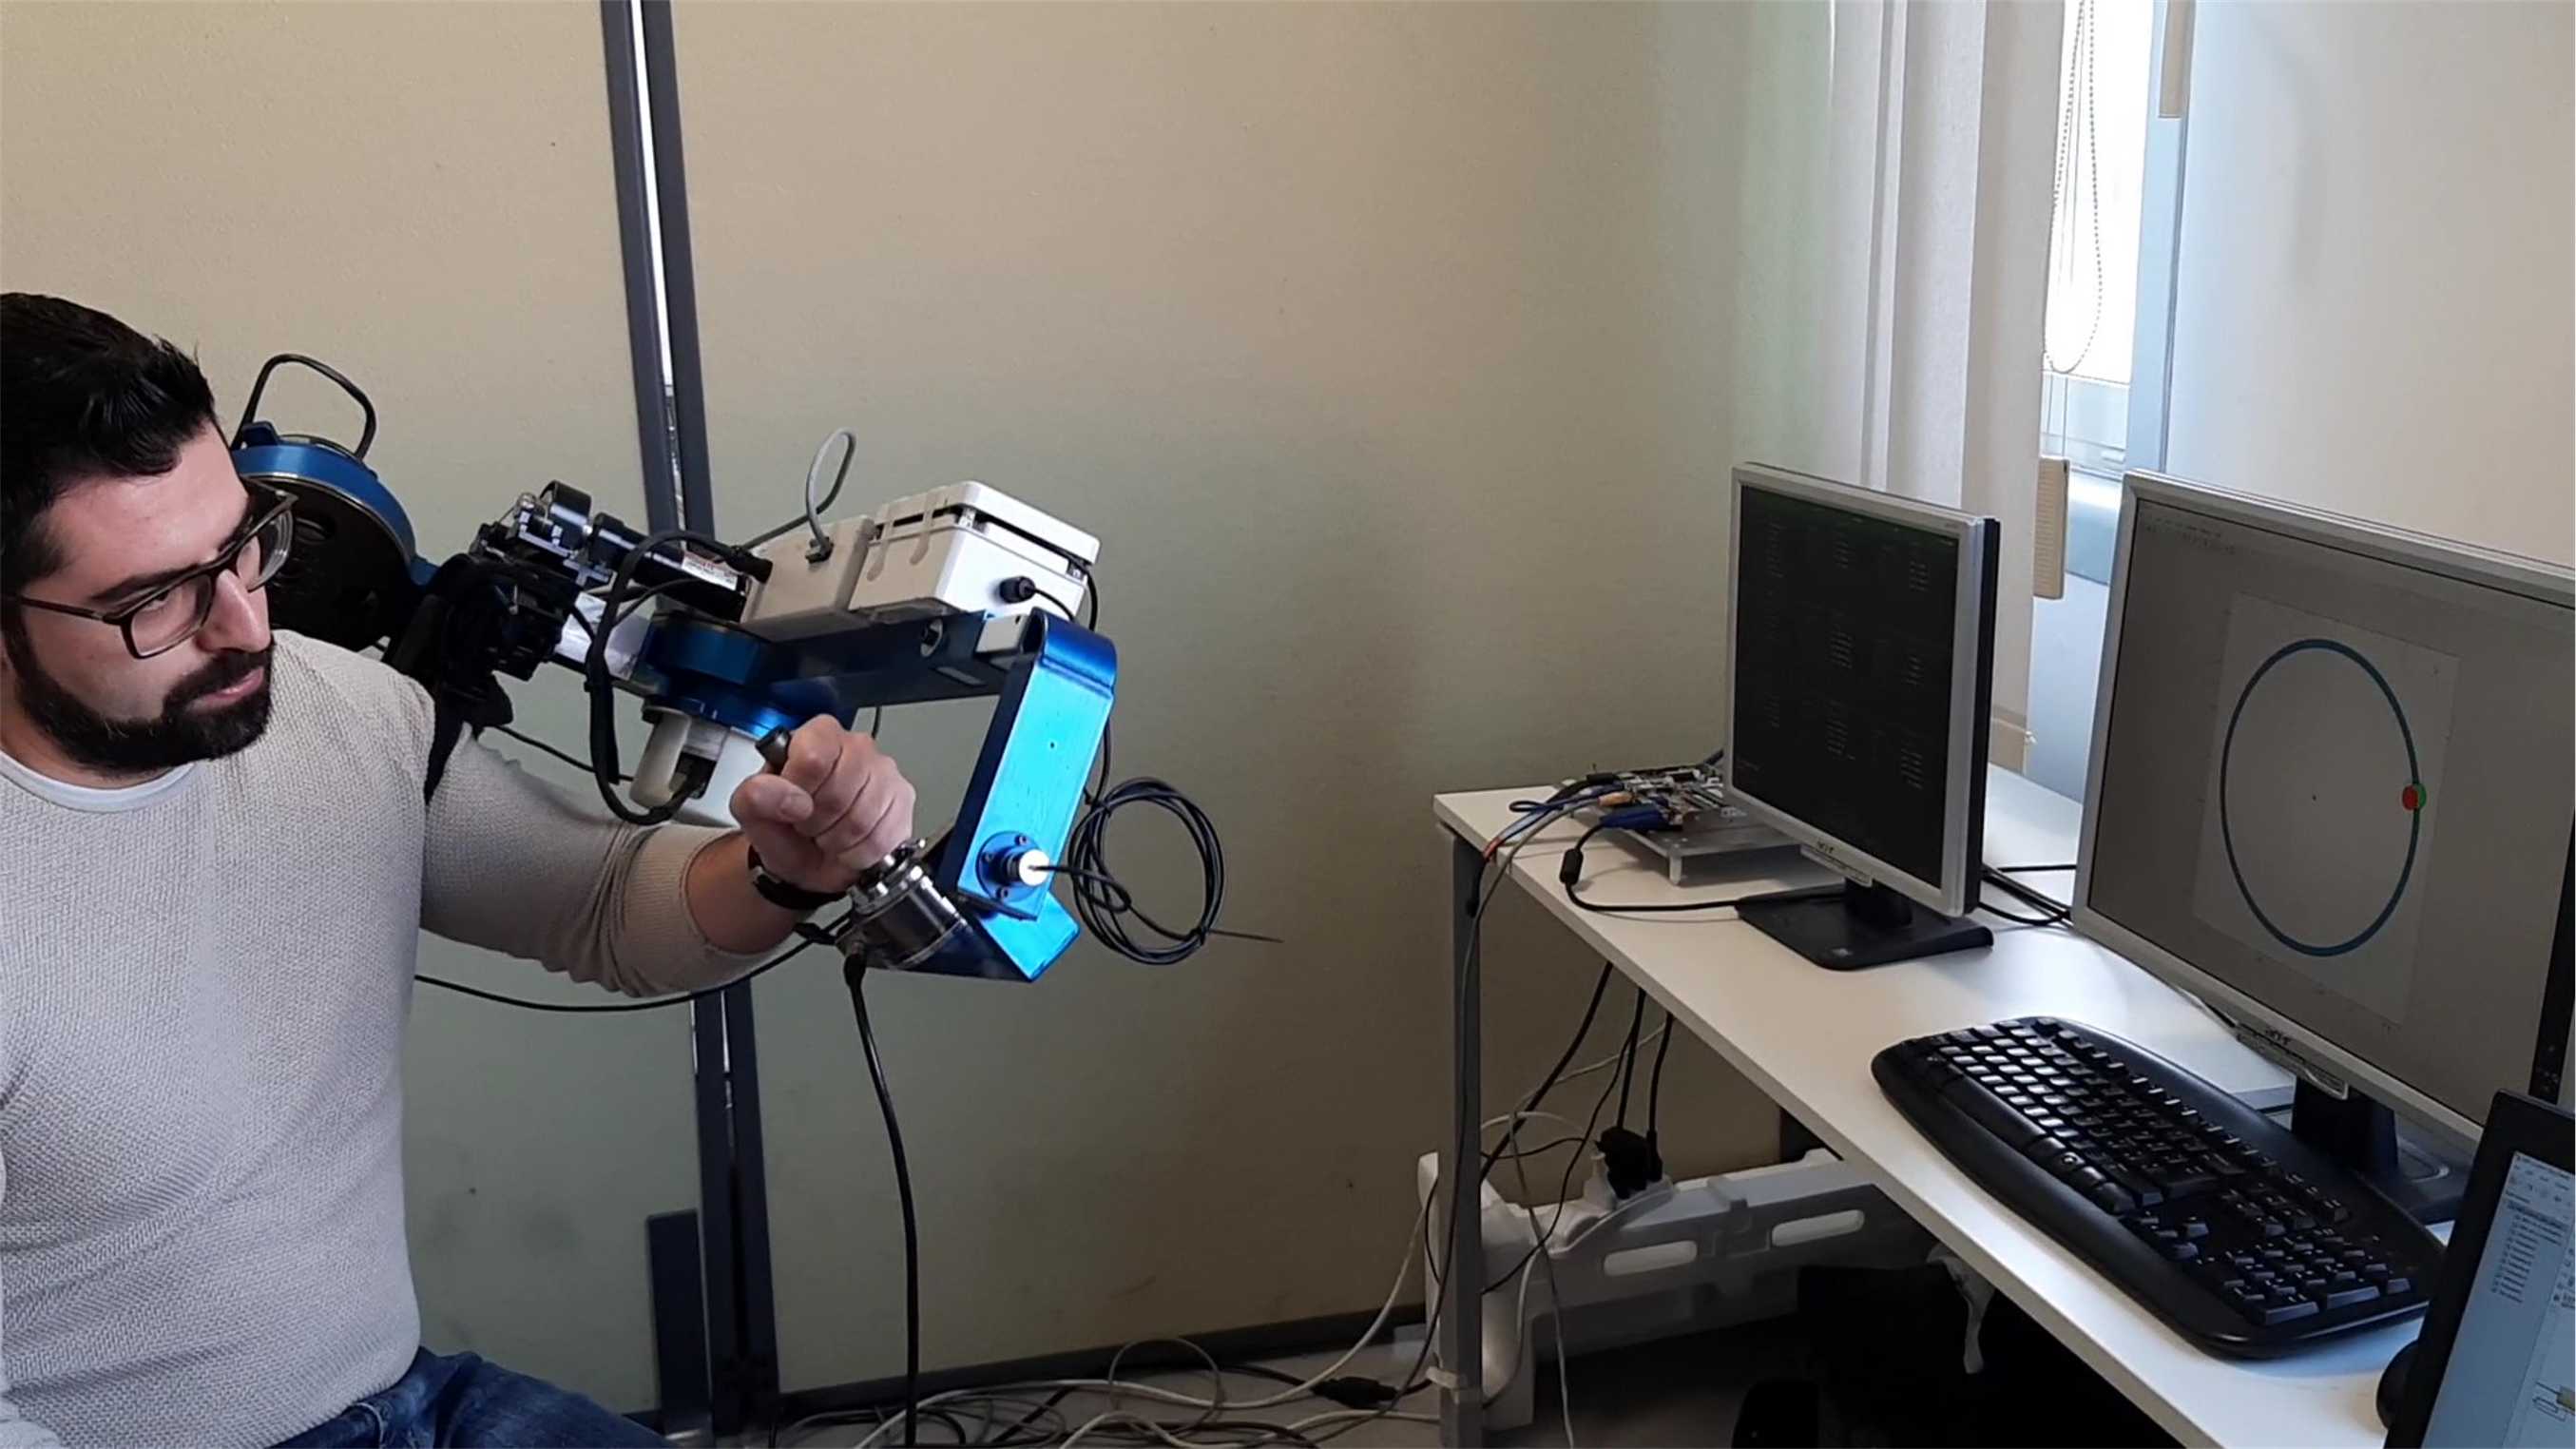
\includegraphics[width=0.5\columnwidth]{../imgRevised/experiment_setup}
	\caption{Experimental setup of the transparency test.}
	\label{fig:experimentalSetup}
\end{figure}

\end{reply}

\shortpoint{ Citations appear adequate. }
\shortreply{ We thank the reviewer for its positive comment, some more citations were added to take into account other reviewers' suggestions.}

\subsection*{Minor}

\shortpoint{ There are numerous grammatical inconsistencies involving the use of
	plurals and prepositions.}
\shortreply{ We thank the reviewer for its careful reading. We proofread the work several times in order to minimize the grammatical errors.}


\shortpoint{Abstract: "for several applications" seems vague and irrelevant in the
	opening sentence.}
\shortreply{ In view of the numerous comments, the abstract was rewritten and this sentence was completely revised.}


\shortpoint{Abstract: influence performances in term of $\rightarrow$ influence performance
	in terms o. Abstract: an other $\rightarrow$ [another]}
\shortreply{ The sentence was rewritten.}


\shortpoint{Abstract: complexity, maximum torque, transparency and haptic
	capabilities $\rightarrow$ complexity, maximum torque, transparency, and haptic
	capabilities
	This is a minor and common mistake, but lists of 3 or more things
	should have a comma also before the "and". Check paper throughout,
	including title. }
\shortreply{ The sentence was rewritten.}


\shortpoint{Some inconsistent formatting, missing plurals, missing oxford commas,
	and incorrect verb tenses (noted in pdf)}
\shortreply{ We thank the reviewer. We try to improve the grammar and fix errors.}
. 

\shortpoint{Some awkward formulation of infinitive verb forms: "allows to obtain"
	should be replaced by "allows it to obtain" or "allows obtaining".
	Check for similar throughout paper, e.g.: 
	capable to exert $\rightarrow$ capable of exerting 
	capable to infer $\rightarrow$ capable of inferring}
\shortreply{ We thank you particularly the reviewer for this suggestion, as this is a common error made by non-native English speaker in the improper usage of allow and capable. This has been fixed.}


\shortpoint{Page 2: awkward phrasing: "for what concern transparency" $-->$
	"regarding transparency"}
\shortreply{ Fixed.}


\shortpoint{Page 2: what does it mean to evaluate at geometrical level the
	quantitative and qualitative behavior of the controller? This portion
	of the introduction is important to provide the user with an
	understandable overview of what's to come. Further effort should be
	made to make the text more reader friendly and less ambiguous.}
\shortreply{ We agree with the reviewer that this sentence was unclear and has been reformulated as follows:
	{\em  As far as haptic rendering, the stability behavior and quality of force rendering of the proposed controller was assessed through a virtual wall simulation implemented with increasing  stiffness values and  compared it with the other two  benchmark controllers.}}


\shortpoint{Page 3: controls $\rightarrow$ "controllers" or "control schemes"}
\shortreply{ This typo has been fixed.}


\shortpoint{Page 3: it seems odd that the value of 3.7 is given for both weight and
	inertia after the reduction. Is this a typo?}
\shortreply{ The correct figure for motor inertia is 2.5. This was corrected in the text.}


\shortpoint{Page 4: why is R defined here in text when not used in the equations
	(1) and (2)?}
\shortreply{ The reviewer is correct, the definition has been removed.}


\shortpoint{Page 4: the strain gauges were placed at a distance of 3mm from the
	extremities. How was this location determined besides just not being in
	the middle and not beign too close to the end?}
\shortreply{ This was estimated by means of FEM and was chosen closer to the ends to maximize sensitivity, but avoiding border effects due to the fillet radius.}


\shortpoint{Fig.8: some small text and the arrow pointing to the location of the
	sensor is not clear. Location of probe is not visible at all in black
	and white.}
\shortreply{ The figure was made again to be more clear.}


\shortpoint{Page 5: avoid using "(n+1)-th" link. Referring to the n-th link is
	okay, but n+1 would be less ambiguous as "link n+1".}
\shortreply{ We agree, the suggested notation was adopted.}


\shortpoint{Page 5: deputed to estimate $\rightarrow$ employed to estimate?}
\shortreply{Thanks, fixed.}


\shortpoint{Figure 12: this is a figure for 3 different joints, but only one curve
	is shown. Do they all have the same curve? Is this just for the motor
	or does it involve the link inertias as the term "Joint" would imply?}
\shortreply{ This involve a single joint mounted on a testbed with a calibrated inertia link mounted on it. The phase diagram was added as well to this figure. An explanation was added in the figure caption as {\em joint sensor torque vs. motor torque command in standardized testbed conditions.}}, while in the text it is stated {\em Considering an average link inertia, it can be obtained the natural frequency for each joint elastic transmission. Results are shown in the}


\shortpoint{Figure 17: it's not clear from the figure if the observations made in
	text are accurate. Although the position and acceleration are similar,
	the plots in (a) and (b) have different scales on both x and y axes
	which could contribute in part to the lower interaction torques. When
	plots are compared, their axes should be scaled equally.}
\shortreply{ Thanks, we agree, the corresponding figures has been now changed. The reviewer will find the new data in figure 14 and 15, where these observations were taken duly into account.}


\shortpoint{Figure 18: it would be nice to see the target circle, perhaps overlaid
	in white, on the plot for reference.}
\shortreply{ This figure was made again, now in figure 12 the suggestion of the reviewer was taken into account.}


\shortpoint{Page 12: few details are provided about the controller evaluation
	trials T1-T4 and the details provided use some ambiguous terms that
	don't help to clarify what was done. Please revise and add text to
	improve the clarity. }
\shortreply{ Fixed.}


\begin{point}
For additional markup and suggested revisions, see attached pdf.
\end{point}
\begin{reply}
The comments in the pdf were also implemented in the revised text. We take the occasion to thank the reviewer for the in-deep revision of the text.
\end{reply}

\setcounter{reviewer}{4}
\reviewersection

% Point one description 


% Point one description 
\begin{point}
While many of the techniques are standard, what is commendable is that
the authors implemented this control architecture in real hardware. The
importance of this should not be understated. This represents a
significant amount of work. With some revisions to enhance the clarity
of the presentation, This could be an impactful paper.
\end{point}

% Our reply
\begin{reply}
	We thank the reviewer for this comment, we agree and we confirm that demonstrating in real hardware requires bigger effort that allows to evaluate experimentally some theoretical assumptions.
	
\end{reply}


\begin{point}

The biggest issue I have with the paper is that the reader has to get
to the end of the paper to discover what the authors' central
contribution is. The thesis of the paper, found in the conclusion, is
that it provides evidence that with a suitable control architecture, it
is not necessary for a rehabilitation upper limb exoskeleton to be
backdrivable by the user. This is important. However, from the start of
the paper, it is not clear where the paper is going. The introduction
is overly long, and cites work only loosely related to the work
presented, e.g. works on lower limb exoskeletons. It then launches into
the (previously published) description of the hardware, and the
narrative as written gives the impression that this is a paper about a
new exoskeleton, when in fact the novelty is the control architecture
for the exoskeleton, particularly a comparative hardware evaluation of
several alternatives. This should be made clear from the outset, even
in the abstract. The abstract should list the types of controllers
evaluated and which was found to be superior in the given context.
\end{point}


\begin{reply}
We followed this important suggestion, that allowed us better focus on the paper.

The introduction was partly rewritten and both abstract and introduction were better focused on the results of the paper.
We agree that were some references that were loosely connected to the actual work, so we shortened some parts were detailed description of other exoskeletons implementation was provided.
\end{reply}


\begin{point}
Throughout the paper, there are some odd choices that were made in the
work. For example, to combat misalignment of the strain gauge on the
spring element of the torque sensor, the authors use a neural network
with training data. There are well-established methods to address this,
such as differential pairs and using a hardware calibration. Why the
neural network? It seems to cost more in the way of development for
something that is less reliable.
\end{point}

\begin{reply}

The neural network is an adaptive modeling approach that without prior knowledge of internal parameters is capable of reaching with only one session of training a good performance. Although we agree with the reviewer that there are more specific methods available in literature, we considered that the ANN approach was more flexible thanks to its adaptivity and due to the complexity of the model we consider that this was an acceptable approximation.  
We added in the text that the clarification that  ANN method was chosen due to its adaptive nature.
\end{reply}



\begin{point}



 The two-mass model in Fig. 11 is used
to approximate the linkages of the robot, but this neglects the dynamic
equations of this links. Some justification might be found for this in
the fact that the gear ratio is on the order of 100, but the authors
make no such justification, then they mention joint torques due to
centripetal and coriolis terms, which would suggest they are including
these terms, but the narrative is ambiguous.
\end{point}



\begin{reply}
We have tried to improve the description of dynamic equations to make more clear all the assumption behind the presentation of our dynamic model.
The link dynamics is modeled completely, taking into account in matrices M and C both inertias and Coriolis effects. In section III.B (equation 10) and in appendix I there is a detailed explanation on how then the dynamics is split into different contributions.
 Of course in the two-mass model of section III.A for each link all the inertias are reduced to the axis of the link, so that only the dynamics acting on the motor axis is considered. 
 The joint coupling is considered in the multi-joint dynamic model in section III.B that is one of the contributions of the paper.
 In equation (9) we have now added some braces that highlight the contribution of both joint and motor dynamics. The compensation of dynamics was verified by the good results obtained in the experimental characterization of transparency.
\end{reply}




\begin{point}

 They speak of a natural
frequency in the discussion around Fig. 12, which suggests a
linearization was performed (where the resonance would shift with
operating point). Fig. 12 shows the magnitude plot but not the phase
plot. The phase would be illustrative of how well the linearization
captures the behavior of the system
\end{point}
\begin{reply}
We agree with the reviewer that the phase plot would be informative, so we have added now the phase plot in the second part of the same figure.
\end{reply}



\begin{point}

 The estimation architecture in
(13) appears to be a predictor architecture only, yet (17) suggests a
sort of Leuenberger Observer architecture (although they call it a
Kalman Filter) No indication of how the observer gains were calculated
or covariance matrices used is given. I am also not clear on why they
needed to observe the joint accelerations to implement the controller.

\end{point}
\begin{reply}

 We have tried to be cleared by adding the following text
 {\em The gain $L$ was found resolving the problem of a Kalman optimum observer based on the experimental covariance data of measurement and process noise. Measurement noise was derived from motor encoder ${\theta}_{m,i}$ measurements, that mainly takes into account the encoder quantization and motor acceleration $\ddot{\theta}_{m,i}$ estimation through (13), thanks to the available torque measurement.}

Actually this is not a reduced observer, but an additional state was added to estimate the motor dynamics. The additional term is used for compensation of motor dynamics.
\end{reply}



\begin{point}
	
	Typically in robotic systems (and others driven by Newtonian Mechanics)
	the acceleration is not a state of the system (unless it happens to
	emerge in place of other positions and velocities by some state
	transformation). The rationale for observing the second derivative is
	not clear. Equation (17) and the surrounding discussion does not help
	the reader evaluate what physical quantities correspond to y (other
	than looking at the products of the state), and in the block diagram on
	the next page it seems that torque is what is measured, so it
	ambiguous.
	
\end{point}
\begin{reply}
A good estimation of the acceleration is crucial to provide dynamics compensation.
More in detail, the estimated joint accelerations have been multiplied by $\hat{M}_i$ that is the inertial term of the i-th joint (the reviewer can find a graphical representation in the new figure 9, at the top-left corner). 
Regarding the block diagram of the old figure 14, the inputs are position and acceleration. To improve clarity, the old figures 13 and 14 has been merged.
\end{reply}




\begin{point}
	It was not clear why in the experiment they had the user
	grab the end effector of the exoskeleton rather than wearing it. If the
	user is wearing the exoskeleton, there would likely be forced applied
	to the various links along their length, which would "break" the
	traditional formulation that depends on computing joint torques through
	the Jacobian transpose, which may call into question some of the
	formulation presented.
\end{point}
\begin{reply}
The user actual wear the exoskeleton, that has two contact points, at arm and level of hand. The dynamic system will lead to compensation of external forces based on the actual readings that are made at level of joint torque sensing.  In equation (23) the effect of additional forces introduced at single points that are not at the end-effector is canceled as an effect of disturbance estimation made by $\tau_{d}$.
In haptic rendering, we expect that forces are rendered at the end-effector.
\end{reply}


\begin{point}
	In section IV, the three controller types are listed, but it would be
	helpful to say, "We evaluated three different controllers". Until the
	end of the narrative, I was under the false impression that the other
	two controllers were embellishments of the first, whereas they were
	three completely disparate solutions.
\end{point}
\begin{reply}
The reviewer is correct, the other 2 controllers have to be considered benchmark architectures. This has been not pointed out since the abstract and in the introduction, so that the reading flow should be significantly improved-
\end{reply}


\begin{point}
	
	By and large the figures are well done. I might suggest that the
	authors display Fig. 21 in three-dimensional space rather than three
	separate curves superimposed on the same plot for each coordinate. 
	
\end{point}
\begin{reply}
This figure has been completely revised, and the plots have been split in different panels to take into account the reviewer suggestion.
\end{reply}


\begin{point}
	
	
	The authors also have several English mistakes that appear throughout,
	for example, using "performances" instead of "performance", and often
	use the wrong preposition in idomatic expressions, e.g. "inspired to"
	rather than "inspired by". There are also several long wordy
	expressions, e.g. "due to the absence of elastic or damping elements",
	which should be expressed more concisely in English, e.g. "which have
	no elastic or damping elements". These are minor, but should be
	resolved in a revision as they disrupt the reader.
\end{point}
\begin{reply}
We thank you the reviewer for pointing out these mistakes, they have been replaced in all occurrences
\end{reply}





\subsection*{Minor}

%% Use the short-hand macros for one-liners.
%\shortpoint{ Typo in line xy. }
%\shortreply{ Fixed.}

\begin{point}
%The authors present a design of a 5-joint, 4 degree of actuation upper
%limb exoskeleton for rehabilitation purposes, with a high gear ratio
%transmission. This makes the exoskeleton non-backdrivable. The main
%contribution is the evaluation of three different control architectures
%for the joints. The authors compare a Full State Feedback Controller, a
%`basic' state feedback controller (a simple proportional-derivative
%task space controller), and a passivity based controller. A summary of
%the hardware design is given, along with an observer architecture to
%estimate the derivatives of the angle from encoder measurements.






Ultimately I believe that a new draft that is tightly focused and
guides the reader to understand the key elements of the work conducted
and its significance throughout the read, rather than finally
understanding during the discussion section, it will be a good paper. \end{point}

% Our reply
\begin{reply}
We thank you very much the reviewer for all the helpful comments. We have now stressed more in the introduction and the paper all the key elements and findings, hoping that will improve paper readability.
 
\end{reply}



%\subsection*{Minor}
%
%% Use the short-hand macros for one-liners.
%\shortpoint{ Typo in line xy. }
%\shortreply{ Fixed.}

\bibliographystyle{apalike}
%\bibliography{references}
\bibliography{../referencesTRO}
%referencesTRO

\end{document}


